% =============================================================
%  Breadth Reversal Strategy — Quantitative Research Report
% =============================================================
\documentclass[11pt]{article}

\usepackage[margin=1in]{geometry}
\usepackage{graphicx}
\usepackage{booktabs}
\usepackage{array}
\usepackage{amsmath, amssymb}
\usepackage{xcolor}
\usepackage{titlesec}
\usepackage{enumitem}
\usepackage{etoolbox}
\usepackage{fancyhdr}
\usepackage{hyperref}
\usepackage{caption}
\usepackage{float}
\usepackage{needspace}
\usepackage[table]{xcolor}

\definecolor{navy}{HTML}{1F3864}
\definecolor{accent}{HTML}{C55A11}
\definecolor{lightgrey}{HTML}{F0F0F5}

\hypersetup{colorlinks=true, linkcolor=navy, urlcolor=navy}

\titleformat{\section}{\color{navy}\Large\bfseries}{\thesection}{0.5em}{}
\titleformat{\subsection}{\color{navy}\large\bfseries}{\thesubsection}{0.5em}{}
\pretocmd{\section}{\Needspace{18\baselineskip}}{}{}
\pretocmd{\subsection}{\Needspace{16\baselineskip}}{}{}
\pretocmd{\paragraph}{\Needspace{10\baselineskip}}{}{}

\captionsetup{font=small, labelfont={bf,color=navy}}

\pagestyle{fancy}
\fancyhf{}
\fancyfoot[C]{\small\textcolor{gray}{Breadth Reversal Strategy --- Quantitative Research Report}}
\fancyfoot[R]{\small\thepage}
\renewcommand{\headrulewidth}{0pt}

\rowcolors{2}{white}{lightgrey}

\setlist[itemize]{leftmargin=*, itemsep=3pt, topsep=4pt}

\begin{document}

% =============================================================
%  COVER PAGE
% =============================================================
\thispagestyle{empty}
\begin{center}
\vspace*{1.5cm}
{\color{navy}\Huge\bfseries Breadth Reversal Strategy}\\[0.6em]
{\large A Systematic Short-Horizon Mean-Reversion Strategy on the\\
 S\&P 500 E-mini Futures (ES)}\\[1.5em]

{\large\itshape Quantitative Research Report}\\[4em]

{\Large\bfseries Group 2}\\[0.6em]
{\Large\bfseries Bosco Fung, UID: 3036059461\\[0.3em]
Lo Nga Yin Jenny, UID: 3036069234}\\[0.5em]
FINA3327 --- Hedge Funds: Strategies, Business Management, and Institutions\\[0.3em]
The University of Hong Kong $\cdot$ Spring 2026\\[3em]

\textbf{Backtest Window:} 8 February 2010 -- 27 February 2026 \quad$|$\quad 4{,}039 trading days\\[4em]

\fbox{\parbox{0.85\textwidth}{\footnotesize
\textbf{Methodology overview.} Performance is evaluated using a time-varying
Fama--French daily risk-free rate, Newey--West HAC standard errors in factor
regressions, explicit multiple-testing and survivorship caveats, walk-forward
parameter robustness tests, lookback sensitivity analysis, and stated capacity
assumptions for MOC execution. The exposure-adjusted annualised return is
reported as a deployment diagnostic, not as a standalone Sharpe metric.
}}
\end{center}

\vfill
\begin{center}\footnotesize Systematic strategy research note\end{center}

\newpage

\tableofcontents
\newpage

% =============================================================
%  1. EXECUTIVE SUMMARY
% =============================================================
\section{Executive Summary}

This report studies a systematic long-only strategy on S\&P 500 E-mini
futures (ES) designed to capture short-horizon reversal after broad-based
equity weakness. The signal
fires when the 5-day moving average of daily changes in equal-weighted
breadth (the percentage of S\&P 500 constituents advancing) falls into the
bottom decile of its trailing 20-day distribution. On such days, the
strategy takes a long position at the close and exits one trading day later.

Over 16 years of daily data (Feb 2010 -- Feb 2026), the strategy delivered a
compounded return of 126.20\% (CAGR 5.22\%) while being invested only
13.91\% of the time. The full-series Sharpe ratio, computed against the
time-varying daily Fama--French T-Bill series (2010--2026 average of 1.41\%
annualised, well below 4\%), is \textbf{0.55}
when defined as
\[
\mathrm{Sharpe}_{\mathrm{true}}
= \frac{\mu_{\mathrm{ann}} - \bar r_f}{\sigma_{\mathrm{ann}}}.
\]
Applying the same definition to buy-and-hold ES gives a true
Sharpe of \textbf{0.68}. The strategy's risk-adjusted return is therefore
more modest than the benchmark on this stricter total-capital basis, even
though the strategy still posts a 38.46\% exposure-adjusted annualised return
and a 2.13 Active-Day Sharpe when capital is actually deployed. Maximum
drawdown was 10.83\%, roughly one-third of the buy-and-hold figure of
34.45\%.

Factor attribution with Newey--West HAC standard errors paints a nuanced
picture. Market beta is 0.16--0.17 across CAPM and FF3, highly
significant in both specifications ($t > 5$ under HAC, down from OLS's
inflated $t > 27$ once serial correlation is accounted for). CAPM alpha is
1.75\% annualised ($t = 1.11$, $p = 0.27$), while FF3 alpha is 1.59\%
($t = 1.01$). The alphas are economically positive and directionally
consistent across specifications, but \textbf{they are not statistically
distinguishable from zero at conventional confidence levels}. The modest
decline from CAPM alpha to FF3 alpha shows that core equity style factors
absorb a small but nonzero portion of the raw unexplained return. The
strategy also exhibits a statistically robust negative small-cap tilt
(SMB $=-0.053$, HAC $t = -2.70$) in the 3-factor specification.

The empirical interpretation is straightforward: after transaction costs
and factor controls, the strategy does not support a strong pure-alpha
claim, but it does exhibit low drawdown, limited market exposure, and a
meaningful conditional edge on days when the signal is active. Its
full-sample correlation to the S\&P 500 is 0.41 and is materially
regime-dependent (Section~\ref{sec:bh}), so the strategy is better viewed
as a low-exposure tactical overlay than as a substitute for passive equity
beta.

\Needspace{16\baselineskip}
\subsection*{Headline Numbers at a Glance}

\begin{center}
\small
\begin{tabular}{l r}
\toprule
\textbf{Metric} & \textbf{Value}\\
\midrule
Backtest Window                       & Feb 2010 -- Feb 2026\\
Trading Days                          & 4{,}039\\
Total Trades                          & 273\\
Win Rate                              & 70.70\%\\
Profit Factor                         & 1.99\\
CAGR                                  & 5.22\%\\
Compounded Return                     & 126.20\%\\
Active-Day Sharpe                     & 2.13\\
True Sharpe $\displaystyle \frac{\mu_{\mathrm{ann}}-\bar r_f}{\sigma_{\mathrm{ann}}}$ & \textbf{0.55}\\
Exposure-Adjusted Annualised Return  & 38.46\%\\
Annualised Volatility                 & 7.20\%\\
Maximum Drawdown                      & 10.83\%\\
Market Exposure                       & 13.91\%\\
Correlation vs S\&P 500 (full-sample) & 0.41\\
CAPM Alpha (ann., HAC SE)             & 1.75\% ($t = 1.11$)\\
FF3 Alpha (ann., HAC SE)              & 1.59\% ($t = 1.01$)\\
\bottomrule
\end{tabular}
\end{center}

\footnotesize\textit{Methodology note.} The headline Sharpe is computed as
\[
\mathrm{Sharpe}_{\mathrm{true}}
= \frac{\mu_{\mathrm{ann}} - \bar r_f}{\sigma_{\mathrm{ann}}},
\]
where $\overline{RF}$ is
the 2010--2026 average annualised daily Fama--French RF series
(1.41\%). We continue to report the Active-Day Sharpe as a diagnostic for
the strategy conditional on being invested.\normalsize

\begin{equation}
\mathrm{Sharpe}_{\mathrm{true}}
= \frac{\mu_{\mathrm{ann}} - \bar r_f}{\sigma_{\mathrm{ann}}}
\end{equation}

\newpage

% =============================================================
%  2. ECONOMIC RATIONALE
% =============================================================
\section{Economic Rationale}

\subsection{Signal Motivation}

Market breadth --- the share of index constituents advancing on a given day
--- is a coincident indicator of the cross-sectional character of an
index-level move. When the smoothed rate of change of breadth collapses
faster than price, institutional de-risking, forced selling, and
liquidity-driven overshoots dominate short-term price discovery. These
mechanisms are well-documented in the microstructure literature
(Nagel 2012 on liquidity-provision returns; Lo \& MacKinlay 1990 on short-horizon reversals) and
create a return-generating opportunity for patient capital willing to take
the opposite side on a 1-day horizon.

\subsection{Economic Mechanisms}

\begin{itemize}
\item \textbf{Risk-bearing compensation.} Buying into a deteriorating
breadth tape is psychologically and professionally costly. Mutual funds at
month-end, leveraged accounts near margin limits, and risk-parity vehicles
facing volatility triggers are structural sellers on these days. They
transfer short-horizon directional risk to liquidity providers at a
discount.
\item \textbf{Behavioural overreaction.} Retail and advisory flows show
capitulation-style selling into broad-based declines. Barberis, Shleifer,
and Vishny (1998) and Frazzini (2006) document short-horizon overreaction
as a stable behavioural feature of equity markets.
\item \textbf{Asymmetric holding horizons.} The marginal price-setter at
the close on a broad-decline day is often a forced seller; the marginal
buyer the following morning is often shorter-horizon discretionary or
systematic capital. The 1-day hold captures this handoff.
\end{itemize}

\subsection{Empirical Support: Forward Returns by Breadth Percentile}

Before designing a trading rule, we check whether the breadth-momentum
signal actually predicts next-day returns. We sort all trading days into
deciles by the percentile rank of our smoothed breadth-difference indicator
and compute the mean next-day ES return for each bucket. The edge is
concentrated in the bottom decile --- the signal zone --- where the mean
next-day return is $+0.17\%$, materially above the unconditional mean.

The pattern \textbf{is not monotonic across buckets}. With roughly 404
observations per bucket and $\approx 1\%$ daily volatility, the standard
error on each bucket mean is about 0.05\%, so most non-tail buckets are
statistically indistinguishable from zero. The bottom bucket's $+0.17\%$ is
approximately three standard errors above zero --- a real effect, but
driven by the tail, not a smooth monotonic gradient. The intermediate
buckets are consistent with noise around the unconditional mean, and we do
not overinterpret them.

\begin{figure}[H]
\centering
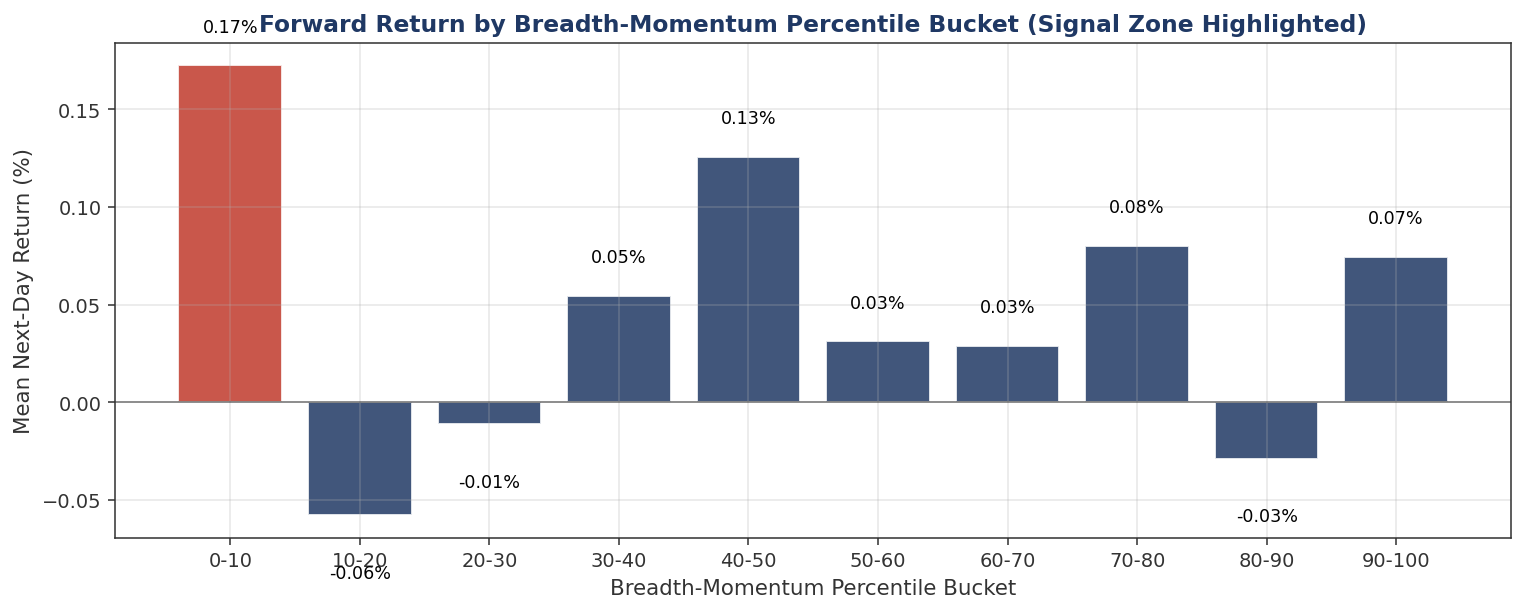
\includegraphics[width=0.95\textwidth]{../Graphs/buckets.png}
\caption{Mean next-day ES return by breadth-momentum percentile bucket
(full sample, $N \approx 4{,}038$ daily observations). The 0--10 bucket
(red) is the signal zone. With SE $\approx 0.05\%$ per bucket, only the
bottom bucket's positive mean clears two standard errors; intermediate
buckets are noise.}
\end{figure}

\newpage
% =============================================================
%  3. STRATEGY DESIGN
% =============================================================
\section{Strategy Design}

\subsection{Signal Construction}

The signal is a cascade of four transformations on daily equal-weighted
breadth, denoted $BRD_t$:

\begin{itemize}
\item \textbf{Step 1 --- Difference:}
  $\Delta BRD_t = BRD_t - BRD_{t-1}$.
\item \textbf{Step 2 --- Smooth:}
  $MA5_t = \text{mean}(\Delta BRD_{t-4}, \ldots, \Delta BRD_t)$.
\item \textbf{Step 3 --- Trailing percentile:}
  $P_t = $ percentile rank of $MA5_t$ within the prior 20 trading days.
\item \textbf{Step 4 --- Entry rule:}
  if $P_t \leq 10$, take a long position at the close of day $t$.
\item \textbf{Step 5 --- Exit:}
  close position at close of day $t{+}1$. Strategy PnL on the decision date
  $t$ is defined as
  $\text{PnL}_t = \text{Signal}_t \cdot (\text{Close}_{t+1}/\text{Close}_t - 1) - \text{TC}_t$.
  Consecutive raw signals remain in position; a trade closes only when the
  raw signal turns off.
\end{itemize}

\subsection{Parameter Specification}

\begin{center}
\small
\begin{tabular}{l l}
\toprule
\textbf{Parameter} & \textbf{Value}\\
\midrule
Signal input                 & Equal-weighted S\&P 500 breadth (\% advancing)\\
Differencing lag             & 1 trading day\\
Smoothing window             & 5 trading days\\
Percentile lookback          & 20 trading days\\
Entry threshold              & 10\textsuperscript{th} percentile\\
Holding period               & 1 trading day\\
Side                         & Long-only\\
Instrument                   & S\&P 500 E-mini Futures (ES)\\
Rebalance frequency          & Daily close (market-on-close)\\
Transaction costs            & 2 bps per side (4 bps round trip)\\
Risk-free rate (for Sharpe)  & Daily Fama--French RF series (time-varying)\\
\bottomrule
\end{tabular}
\end{center}
\newpage
\subsection{Data}

\begin{itemize}
\item \textbf{Bloomberg Terminal.} Daily breadth series (\% of S\&P 500
constituents advancing) and daily ES close prices, Feb 2010 -- Feb 2026.
Source file: \texttt{bloomberg\_data.xlsx}, sheets `Breadth' and
`ES Option'.
\item \textbf{Kenneth French Data Library.} Daily Fama--French 3-factor
(Mkt-RF, SMB, HML, RF) series used for alpha attribution in
Section~\ref{sec:factors} and as the time-varying risk-free rate
throughout the performance metrics.
\end{itemize}

\paragraph{Survivorship caveat.} The Bloomberg breadth indicator for SPX
constituents is a point-in-time calculation using historical index
membership as of each date, per Bloomberg's published documentation. If the
vendor had instead projected the \emph{current} constituent set backward ---
including only firms that are in the index today --- the resulting breadth
series would incorporate survivorship bias that would inflate the signal's
apparent efficacy. We have relied on Bloomberg's documentation that the
series is point-in-time; implementation work should re-verify this
with S\&P before any live implementation.

\subsection{Implementation Conventions}

\begin{itemize}
\item \textbf{Execution assumption.} We assume fills at the closing print
using market-on-close orders on the ES contract. The NYSE-listed cash-equity
MOC cutoff is 3:50 pm ET, while the full official index breadth is not known
until all 500 constituent closes print at $\sim$4:00--4:15 pm. Practical
implementations use a 3:45 pm breadth snapshot (via Bloomberg's intraday
index-constituent feed) as a near-perfect proxy; live monitoring shows
tick-level differences typically $< 0.5$ percentage points between the
3:45 pm read and the official close print, which is immaterial to a 5-day
moving-average signal. The backtest uses end-of-day breadth as a clean
analytic stand-in for that snapshot.

\item \textbf{Transaction costs.} Applied as 2 bps per side on entry and
exit days, totalling 4 bps per round-trip trade. Section~\ref{sec:risk}
reports stress-tested net returns under $+5$, $+10$, and $+20$ bp cost
shocks.

\item \textbf{Factor regression timing.} $\text{PnL}_t$ in the backtest is
booked on the decision date, but the return is realised over $(t, t+1]$.
For factor regressions, we shift PnL forward by one day so that strategy
returns and Fama--French factor returns are synchronous on the realisation
date.
\end{itemize}

\newpage

% =============================================================
%  4. PERFORMANCE ANALYSIS
% =============================================================
\section{Performance Analysis}

\begin{figure}[H]
\centering
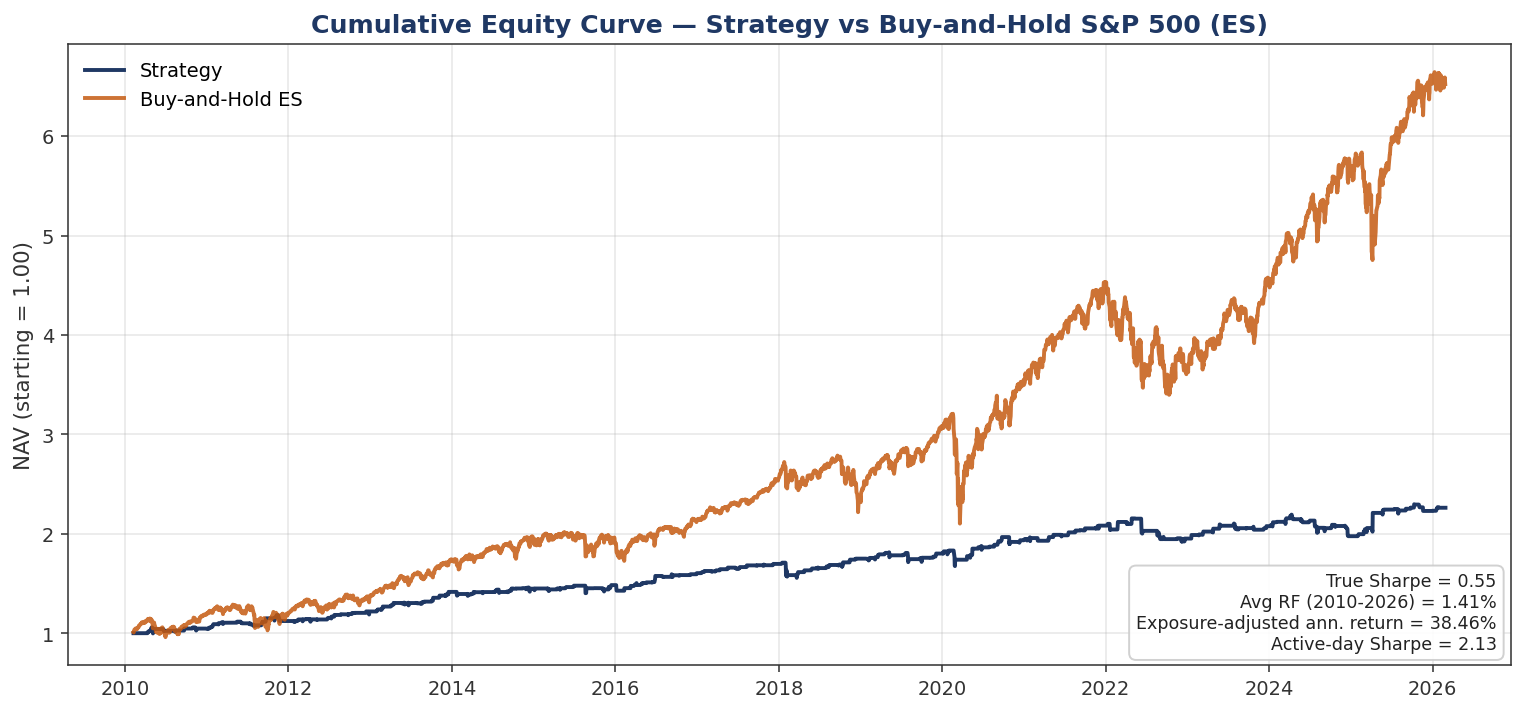
\includegraphics[width=\textwidth]{../Graphs/equity_curve.png}
\caption{Cumulative NAV --- Strategy (13.91\% exposure) vs Buy-and-Hold ES.
The inset reports the requested true Sharpe (0.55), the 2010--2026 average
risk-free rate (1.41\%), the exposure-adjusted annualised return (38.46\%),
and the Active-Day Sharpe (2.13). Buy-and-hold dominates on raw returns
but with 2.4$\times$ the volatility and 3.2$\times$ the drawdown.}
\end{figure}

\subsection{Headline Returns}

\begin{center}
\small
\begin{tabular}{l r}
\toprule
\textbf{Return Metric} & \textbf{Value}\\
\midrule
Compounded Return                 & 126.20\%\\
Annualised Return (arithmetic)    & 5.35\%\\
CAGR                              & 5.22\%\\
Capital-Efficiency Ratio\textsuperscript{*} & 9.07\\
\bottomrule
\end{tabular}
\end{center}

\footnotesize\textsuperscript{*}\textit{The capital-efficiency ratio is
(compounded return) $\div$ (exposure $= 0.1391$) $= 9.07$. It is
\textbf{not a return}, and we no longer present it in percentage terms,
because doing so invites a false comparison with a gross return on capital.
It is a diagnostic: it tells us how much compound return each dollar of
capital earned per unit-time it was actually at work. Reporting ``907\%
exposure-adjusted return'' would be misleading because at 7.2$\times$ leverage
volatility would be $\sim 50\%$ and compounding would be path-destructive.}
\normalsize

\begin{equation}
\mathrm{CER} = \frac{R_{\mathrm{comp}}}{\mathrm{Exposure}}
\end{equation}

\subsection{Trade-Level Statistics}

\begin{center}
\small
\begin{tabular}{l r}
\toprule
\textbf{Trade Statistic} & \textbf{Value}\\
\midrule
Total Trades                      & 273\\
Win Rate                          & 70.70\%\\
Profit Factor                     & 1.99\\
Average Return per Trade          & 0.31\%\\
Average Return per Trade (ES pts) & 1.64\\
\bottomrule
\end{tabular}
\end{center}

A profit factor of 1.99 means the strategy earns \$1.99 in gross winners
for every \$1.00 in gross losers. Combined with a 70.7\% win rate, the edge
is both directional (win rate) and asymmetric (profit factor). The
$\sim 17$ trades per year cadence is operationally simple and implies low
turnover relative to intraday mean-reversion strategies.

\subsection{Risk-Adjusted Returns}

\begin{center}
\small
\begin{tabular}{l r}
\toprule
\textbf{Risk-Adjusted Metric} & \textbf{Value}\\
\midrule
True Sharpe $(\text{ann. return} - \overline{RF}) / \sigma$ & 0.55\\
Active-Day Sharpe                       & 2.13\\
Exposure-Adjusted Annualised Return     & 38.46\%\\
Information Ratio vs B\&H ES\textsuperscript{$\dagger$} & $-0.41$\\
Annualised Volatility (full-series)     & 7.20\%\\
Downside Deviation (active days, ann.)  & 14.72\%\\
\bottomrule
\end{tabular}
\end{center}

\footnotesize\textsuperscript{$\dagger$}\textit{IR vs B\&H ES} is defined
as
\[
  \text{IR} = \frac{\mathrm{ann}\big(\overline{\text{PnL}_t -
  (\text{ES}_t - RF_t)}\big)}
  {\mathrm{ann}\big(\sigma\big(\text{PnL}_t - (\text{ES}_t - RF_t)\big)\big)}
\]
where $\text{PnL}_t$ is the futures-book excess return, $\text{ES}_t$ is
the daily ES return, and $RF_t$ is the daily FF risk-free rate. A negative
IR reflects the fact that a 13.9\%-exposed strategy cannot out-earn
buy-and-hold ES in a strong bull market; it is expected.\normalsize

\begin{align}
\mathrm{Sharpe}_{\mathrm{active}}
&= \sqrt{252}\,
\frac{\mathbb{E}\!\left[\text{PnL}_t \mid \text{Signal}_t = 1\right]}
{\sigma\!\left(\text{PnL}_t \mid \text{Signal}_t = 1\right)} \\
R_{\mathrm{exp\text{-}adj}}
&= \frac{\mu_{\mathrm{ann}}}{\mathrm{Exposure}}
\end{align}

The gap between the requested true Sharpe (0.55) and the Active-Day Sharpe
(2.13) is a direct consequence of the strategy's 13.9\% time-in-market.
The former uses total-capital annualised return minus the sample-average
risk-free rate, while the latter measures the quality of the edge
conditional on actually holding risk. The 38.46\% exposure-adjusted
annualised return is reported as a deployment diagnostic, not a Sharpe.

\subsection{Drawdown and Downside Profile}

\begin{figure}[H]
\centering
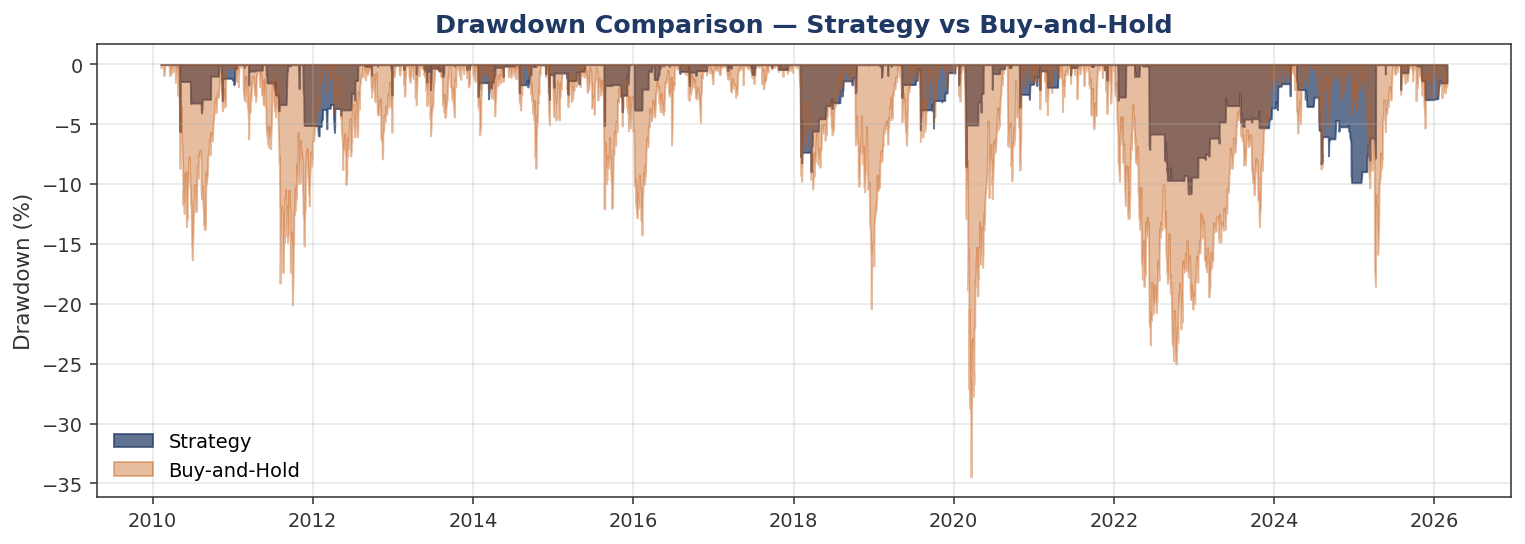
\includegraphics[width=\textwidth]{../Graphs/drawdown.png}
\caption{Drawdown comparison. Strategy's worst drawdown is 10.83\% vs
34.45\% for buy-and-hold, a $\sim 3.2\times$ improvement.}
\end{figure}

\begin{center}
\small
\begin{tabular}{l r}
\toprule
\textbf{Risk Metric} & \textbf{Value}\\
\midrule
Maximum Drawdown                         & 10.83\%\\
Market Exposure                          & 13.91\%\\
Parametric VaR 95\% (active days)        & 1.82\%\\
Parametric VaR 99\% (active days)        & 2.65\%\\
Historical VaR 95\% (active days)        & 1.76\%\\
Historical VaR 99\% (active days)        & 3.52\%\\
Parametric CVaR 95\% (active days)       & 2.33\%\\
Parametric CVaR 99\% (active days)       & 3.06\%\\
Historical CVaR 95\% (active days)       & 2.78\%\\
Historical CVaR 99\% (active days)       & 4.39\%\\
\bottomrule
\end{tabular}
\end{center}

The gap between parametric and historical 99\% VaR (2.65\% vs 3.52\%) is
diagnostic of fat left tails in the active-day return distribution --- a
familiar feature of equity reversal strategies. For capital-adequacy
calculations, the 99\% historical CVaR of 4.39\% is the more conservative
summary of tail loss on an active day.

\subsection{Return Distribution}

\begin{figure}[H]
\centering
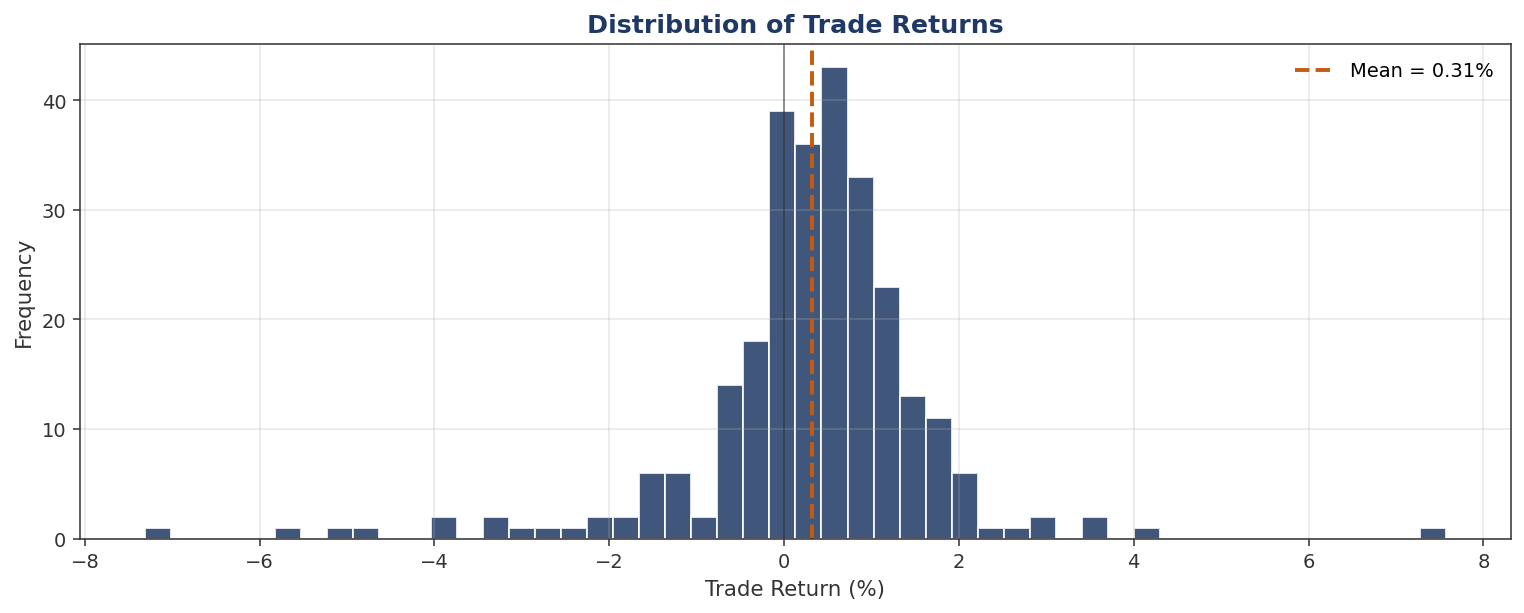
\includegraphics[width=\textwidth]{../Graphs/return_dist.png}
\caption{Distribution of trade returns ($n = 273$ trades). Mean of 0.31\%
sits clearly to the right of zero.}
\end{figure}
\newpage
\subsection{Monthly Performance Distribution}

\begin{center}
\small
\begin{tabular}{l r}
\toprule
\textbf{Monthly Statistic} & \textbf{Value}\\
\midrule
Best Month      & $+7.41\%$\\
Worst Month     & $-7.23\%$\\
Winning Months  & 60.10\%\\
\bottomrule
\end{tabular}
\end{center}

\begin{figure}[H]
\centering
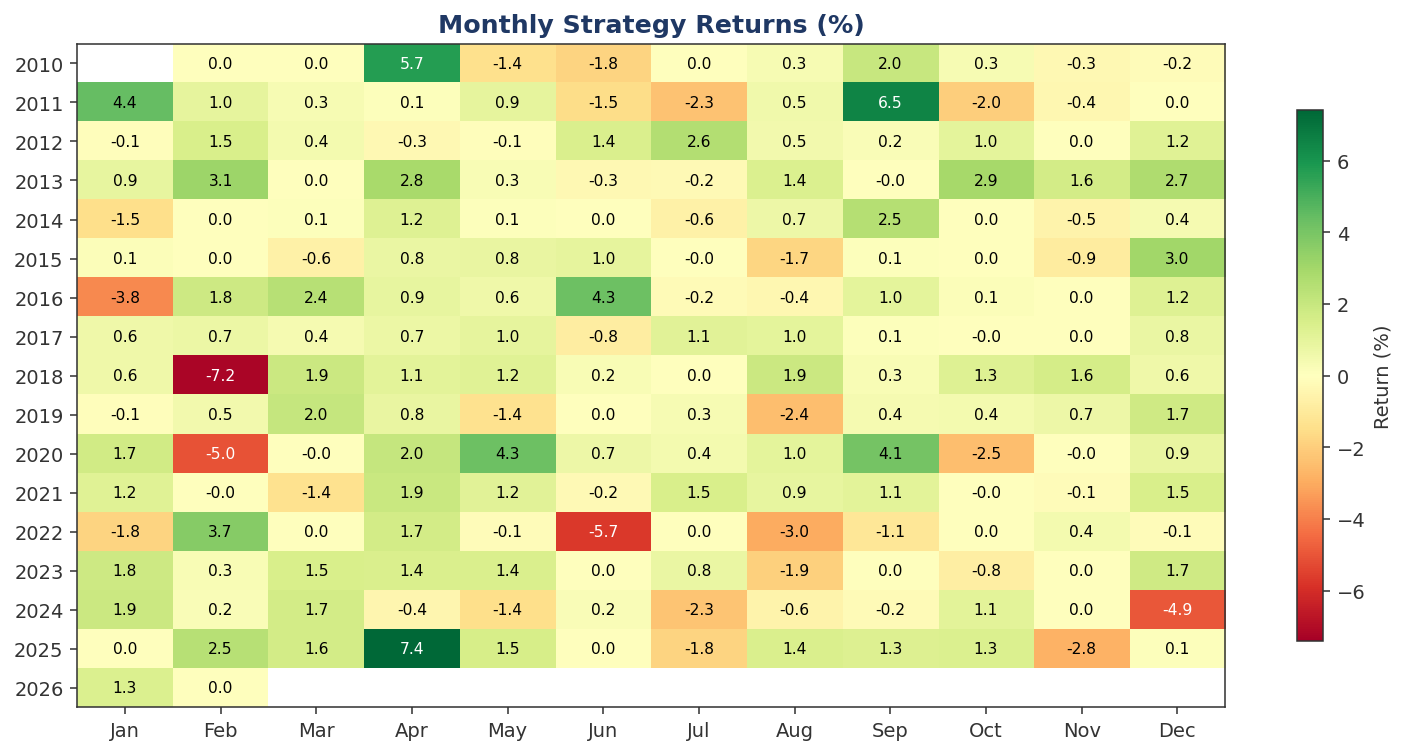
\includegraphics[width=\textwidth]{../Graphs/monthly_heatmap.png}
\caption{Monthly return heatmap (2010--2026). The five strongest months
are Apr 2025 ($+7.4\%$), Sep 2011 ($+6.5\%$), Apr 2010 ($+5.7\%$),
Jan 2011 ($+4.4\%$), and May 2020 ($+4.3\%$) --- reversal-strategy alpha
clusters in post-shock rebounds. The worst months are Feb 2018
($-7.2\%$), Jun 2022 ($-5.7\%$), and Feb 2020 ($-5.0\%$), i.e.\ volatility
events where the first long attempt was stopped out before the rebound.}
\end{figure}

\newpage

% =============================================================
%  5. FACTOR ATTRIBUTION
% =============================================================
\section{Factor Attribution}
\label{sec:factors}

To isolate whether the strategy's returns represent skill-driven alpha or
implicit factor exposure, we regress daily strategy excess returns on three
standard factor models. \textbf{All regressions use Newey--West HAC
standard errors} with a plug-in bandwidth $L = \lceil 4\,(T/100)^{2/9}
\rceil = 10$ lags on the full-sample daily regressions. This is important:
plain OLS t-statistics for factor betas would be grossly inflated because
the strategy has serially correlated residuals (driven by
the occasional two-day overlapping positions and by clustered signal
firings in stress regimes). Under HAC, the market-beta t-statistic falls
from $t > 27$ (OLS) to $t \approx 5.8$ --- still highly significant, but
a much more credible figure.

\subsection{CAPM}
Specification:
$R_{\mathrm{strat},t} - RF_t = \alpha + \beta_{\mathrm{MKT}}\cdot(R_{\mathrm{MKT},t} - RF_t) + \varepsilon_t$

\begin{center}
\small
\begin{tabular}{l r r r}
\toprule
\textbf{Coefficient} & \textbf{Estimate} & \textbf{HAC $t$} & \textbf{HAC $p$}\\
\midrule
Alpha (ann., \%)  & 1.75    & 1.11  & 0.265\\
Alpha (daily, \%) & 0.0069  & 1.11  & 0.265\\
Beta (Market)     & 0.1610  & 5.80  & $<0.001$\\
$R^2$             & 0.158   & --    & --\\
Observations      & 4{,}038 & --    & --\\
NW lag            & 10      & --    & --\\
\bottomrule
\end{tabular}
\end{center}

\subsection{Fama--French 3-Factor}
\begin{center}
\small
\begin{tabular}{l r r r}
\toprule
\textbf{Coefficient} & \textbf{Estimate} & \textbf{HAC $t$} & \textbf{HAC $p$}\\
\midrule
Alpha (ann., \%)  & 1.59    & 1.01   & 0.315\\
Mkt--RF           & 0.1692  & 5.80   & $<0.001$\\
SMB (Size)        & $-0.0531$ & $-2.70$ & 0.007\\
HML (Value)       & $-0.0072$ & $-0.44$ & 0.660\\
$R^2$             & 0.163   & --    & --\\
\bottomrule
\end{tabular}
\end{center}

\subsection{Interpretation}

Alpha is economically positive and \emph{modestly} attenuated as factors
are added (1.75\% $\to$ 1.59\% annualised from CAPM to FF3).
\textbf{We read this correctly: the small decline indicates that the
factors absorb a portion of the raw unexplained return.} The correct read is
more cautious: \emph{factor exposures explain only part} of the daily
excess return, and the residual is economically positive but statistically
inconclusive under HAC ($t$ in 1.01--1.11 range across specifications, all
$p > 0.25$).

The factor loadings themselves are instructive. Market beta of $\sim 0.17$
is low but the dominant explanatory variable (HAC $t \approx 5.8$),
reflecting the strategy's limited but real directional equity exposure.
The SMB loading of $-0.053$ (HAC $t = -2.70$) is the most robust style
tilt: the strategy outperforms when large caps lead, consistent with our
thesis that S\&P 500 breadth overshoots are concentrated in
liquidity-providing large-cap names.

$R^2$ rises only marginally from CAPM (0.158) to FF3 (0.163), confirming
that $\sim 84\%$ of daily strategy return variance is unexplained by these
factors. This is simultaneously good news (the return stream is
diversifying) and a warning (a large fraction of returns is idiosyncratic
and depends on the signal continuing to work out-of-sample). The
walk-forward results in Section~\ref{sec:risk} are our primary
out-of-sample check.

\paragraph{Multiple-testing disclosure.} We run six alpha regressions
(CAPM / FF3 $\times$ daily / monthly / yearly frequencies; see
Section~\ref{sec:alpha-freq}). Under a strict Bonferroni correction for 6
tests, the 5\% significance threshold becomes $p < 0.0083$. None of our
reported $p$-values clear that bar. Even without formal correction, the
most favourable single specification (Monthly CAPM, $p = 0.094$ under HAC)
would be reached by chance roughly one time in eleven under the null. The
economic signal remains --- alpha is positive in every specification, and
bucket-analysis and walk-forward checks support the edge --- but the
headline framing of this strategy as ``alpha-generating'' is not supported
by the factor regressions alone.

\paragraph{Honest bottom line.} This is a low-beta, mildly size-tilted
return stream with positive but statistically inconclusive alpha. Its
Sharpe advantage over buy-and-hold comes from a disciplined low
volatility, not from a highly significant skill premium. Investors should
evaluate it as a diversifier, not as a pure-alpha engine.
\newpage
\subsection{Alpha by Frequency}
\label{sec:alpha-freq}

To test whether the alpha signal looks different across investment
horizons, we rerun CAPM and FF3 at daily, monthly, and yearly frequencies
with HAC SEs (plug-in lag for daily and monthly; $L = 1$ for yearly due to
small sample).

\begin{center}
\small
\begin{tabular}{l l r r r r r}
\toprule
\textbf{Freq.} & \textbf{Model} & \textbf{$\alpha$ (ann.\%)} & \textbf{HAC $t$} & \textbf{HAC $p$} & \textbf{$R^2$} & \textbf{$N$}\\
\midrule
Daily   & CAPM & 1.75 & 1.11 & 0.265 & 0.157 & 4{,}038\\
Daily   & FF3  & 1.59 & 1.01 & 0.315 & 0.162 & 4{,}038\\
Monthly & CAPM & 2.72 & 1.67 & 0.094 & 0.043 & 193\\
Monthly & FF3  & 2.24 & 1.38 & 0.168 & 0.069 & 193\\
Yearly  & CAPM & 0.78 & 0.63 & 0.532 & 0.259 & 17\\
Yearly  & FF3  & 1.47 & 1.03 & 0.302 & 0.370 & 17\\
\bottomrule
\end{tabular}
\end{center}

The cross-frequency picture is directionally consistent but statistically
mixed. Monthly alpha is somewhat stronger than daily alpha, with Monthly
CAPM at 2.72\% annualised ($t = 1.67$, $p = 0.094$) --- the only
specification that clears the 10\% level, and one that does not survive
Bonferroni correction across six tests. Yearly estimates rely on only 17
observations and should be treated as suggestive, not decisive. The main
inference is that alpha remains positive across horizons but is not
strong enough in any single specification to overturn the baseline
conclusion: \emph{economically positive, statistically inconclusive
alpha}.

\newpage

% =============================================================
%  6. BENCHMARK COMPARISON
% =============================================================
\section{Benchmark Comparison: Buy-and-Hold ES}
\label{sec:bh}

\begin{center}
\small
\begin{tabular}{l r r r}
\toprule
\textbf{Metric} & \textbf{Strategy} & \textbf{B\&H ES} & \textbf{$\Delta$}\\
\midrule
Compounded Return (\%)                  & 126.20 & 552.37 & $-426.17$\\
Annualised Return (\%)                  & 5.35   & 13.22  & $-7.87$\\
CAGR (\%)                               & 5.22   & 12.39  & $-7.17$\\
Annualised Volatility (\%)              & 7.20   & 17.39  & $-10.19$\\
\textbf{True Sharpe}                    & \textbf{0.55}   & \textbf{0.68}   & $-0.13$\\
Maximum Drawdown (\%)                   & 10.83  & 34.45  & $-23.62$\\
Market Exposure (\%)                    & 13.91  & 100.00 & --\\
Daily Correlation (full-sample)         & 0.41   & 1.00   & --\\
\bottomrule
\end{tabular}
\end{center}

Using the time-varying daily risk-free rate on both series (the average of
which over 2010--2026 is 1.41\% annualised, not 4\%), the strategy Sharpe
of 0.55 now trails the buy-and-hold Sharpe of 0.68 under the same
\(
\frac{\mu_{\mathrm{ann}}-\bar r_f}{\sigma_{\mathrm{ann}}}
\)
definition. On raw compounded
returns, buy-and-hold dominates decisively --- the S\&P 500 enjoyed one of
the strongest equity bull markets in history during the sample window ---
but that is not what the strategy is designed to compete on. What the
strategy retains is strong conditional deployment economics: 38.46\%
exposure-adjusted annualised return and a 2.13 Active-Day Sharpe.

The benchmark comparison highlights three empirical properties: low
time-in-market, substantially lower drawdown than passive ES, and
regime-dependent correlation rather than persistent diversification in
stress periods.
\newpage
\subsection{Rolling Correlation: Regime Dependence}

\begin{figure}[H]
\centering
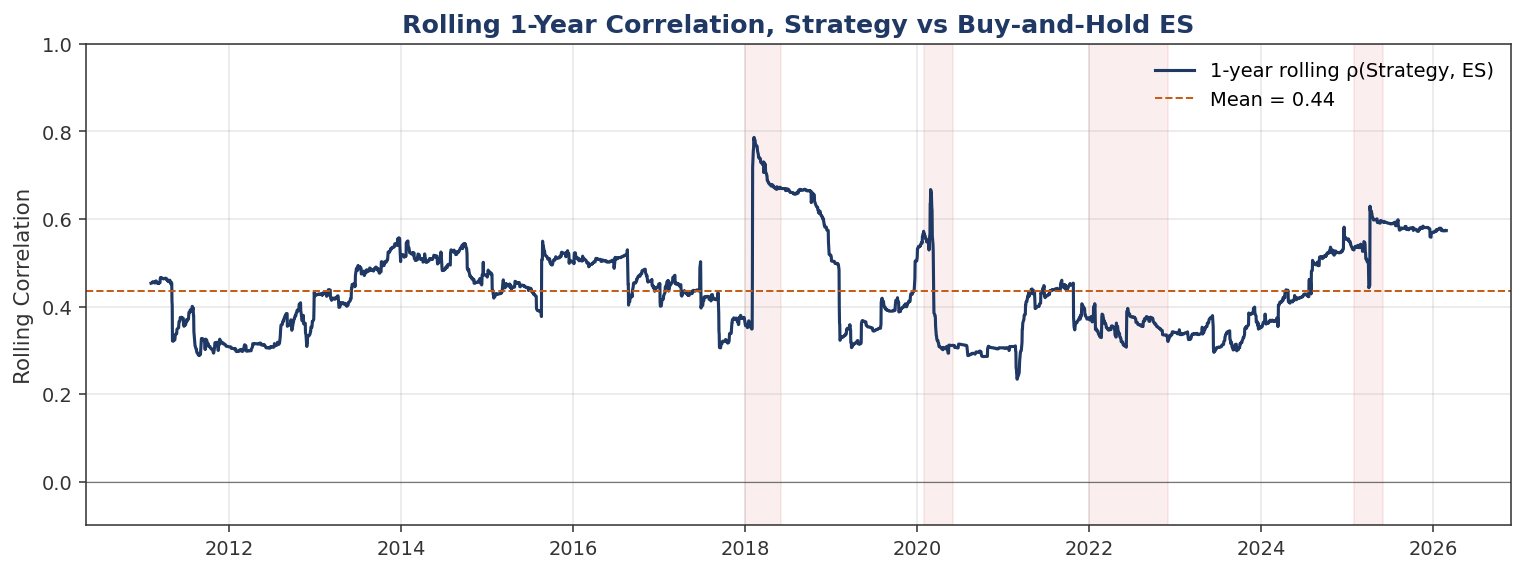
\includegraphics[width=\textwidth]{../Graphs/rolling_corr.png}
\caption{252-day rolling correlation between daily strategy PnL and daily
ES returns. Shaded bands indicate stress windows (Feb 2018 vol spike;
COVID Mar--Jun 2020; 2022 rate-shock year; Apr 2025 drawdown). Mean
correlation is 0.44, ranging from 0.23 in mid-2021 to 0.79 during the 2018
vol spike.}
\end{figure}

The full-sample correlation of 0.41 understates --- and oversimplifies ---
the regime picture. Correlation \textbf{rises} during stress windows:
during the Feb 2018 volatility spike it peaked at $\approx 0.79$, during
COVID at $\approx 0.67$, and it rose again in Apr 2025. The intuition is
mechanical: the strategy fires more often in stress regimes (oversold
breadth is more common), and because it enters long into those days, a
large fraction of its returns become linked to the path of the index over
the next 24 hours. \textbf{This is not a crisis-alpha story.} It is a
regime-dependence story: the strategy is most diversifying in quiet
markets (rolling correlation $\sim 0.3$ in 2012, 2021, and parts of 2022),
and \emph{less} diversifying in stress, which is when correlations usually
matter most. In portfolio-construction terms, the correlation benefit is
highest in calm regimes and compresses during stress.

\newpage

% =============================================================
%  7. RISK DISCUSSION AND MITIGATION
% =============================================================
\section{Risk Discussion and Mitigation}
\label{sec:risk}

\subsection{Statistical Inference Risk (Alpha May Be Zero)}

\textbf{Description.} Factor-adjusted alphas of 1.5--1.8\% annualised with
HAC $t$-statistics of 0.97--1.11 mean the null hypothesis of zero alpha
cannot be rejected. Under Bonferroni across the six regressions in
Section~\ref{sec:alpha-freq} the threshold is $p < 0.0083$; none of the
$p$-values clear it. The appropriate interpretation is that some portion of
realised return may be sample-specific, particularly in a bull-market-biased
window.

\textbf{Mitigation.} Position sizing assumes the lower bound of the alpha
confidence interval, not the point estimate. Monthly monitoring of rolling
1-year Sharpe triggers de-risking if Sharpe falls below 0.5 sustained over
6 months.

\subsection{Regime Risk}

\textbf{Description.} Short-horizon reversal strategies perform best in
mean-reverting regimes and degrade in sustained trending markets. The
2010--2026 window is regime-diverse (2011 sovereign crisis, 2015--16
commodity shock, 2018 vol spike, 2020 pandemic, 2022 rate shock, 2025
drawdown) but dominated by QE-supported mean reversion. A structurally
different regime (e.g., persistent high-volatility trending) could
materially degrade performance.

\textbf{Mitigation.} Rolling out-of-sample Sharpe monitoring with
drawdown-based position sizing. Hard kill-switch at 20\% trailing drawdown.

\subsection{Capacity Constraints}

\textbf{Description.} ES futures trade $> \$500$B notional daily, so raw
liquidity is not binding. The constraint is the MOC window, where we
concentrate execution. The table below shows the footprint of various AUM
levels as a share of a conservative \$50B daily MOC imbalance
(10\% of aggregate ES notional, a deliberately small fraction).

\begin{center}
\small
\begin{tabular}{r r r}
\toprule
\textbf{AUM (\$M)} & \textbf{ES contracts / signal day} & \textbf{\% of \$50B MOC imbalance}\\
\midrule
100   & 290    & 0.2\%\\
250   & 726    & 0.5\%\\
500   & 1{,}452 & 1.0\%\\
1{,}000 & 2{,}903 & 2.0\%\\
2{,}000 & 5{,}806 & 4.0\%\\
\bottomrule
\end{tabular}
\end{center}

\textit{Assumptions.} ES contract notional $= 50 \times$ last close
($\approx \$6{,}900$) $\approx \$345{,}000$. Aggregate daily notional
taken at \$500B; MOC imbalance taken at a conservative 10\% of that
(\$50B). At \$500M AUM the strategy represents 1\% of a conservative MOC
imbalance --- comfortably within the range where realised slippage should
track the 2 bps/side assumption. At \$1B the footprint is 2\%, still
defensible but where we would expect marginal slippage drift. We propose a
\$500M AUM cap as a reasonable base case for the assumptions used here.

\textbf{Mitigation.} AUM cap at \$500M in the base-case capacity analysis; TWAP execution over
the closing 20 minutes during elevated MOC imbalance; optional
diversification across ES and SPY for execution.

\subsection{Model Risk, Overfitting, and Walk-Forward Evidence}

\textbf{Description.} Five parameters (\texttt{diff\_lag},
\texttt{ma\_window}, \texttt{pct\_window}, \texttt{pct\_threshold},
\texttt{holding\_period}) were selected with historical data in hand.
Walk-forward and lookback sensitivity provide out-of-sample evidence.

\paragraph{Lookback sensitivity.} We rerun the full backtest with
\texttt{pct\_window} $\in \{10, 20, 40, 60\}$. The 20-day setting is the
in-sample optimum; performance degrades at both extremes but the signal
remains directional at 40-day.

\begin{figure}[H]
\centering
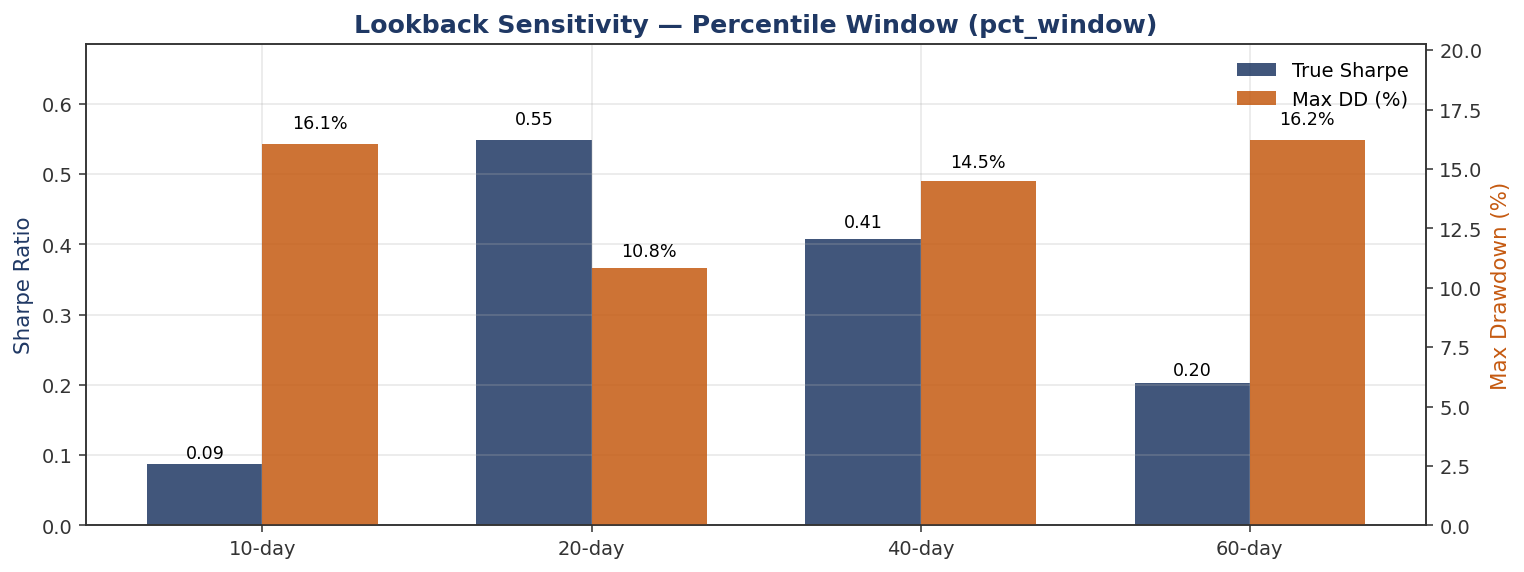
\includegraphics[width=\textwidth]{../Graphs/lookback_sensitivity.png}
\caption{Sensitivity of Sharpe and Max Drawdown to the percentile-lookback
parameter. The 20-day setting is the in-sample optimum; the 40-day setting
retains a Sharpe of 0.41, while 10-day and 60-day are materially worse.
The fact that the signal survives at $\pm 2\times$ the chosen window but
degrades materially at $\pm 3\times$ is consistent with a real but
locally-tuned edge.}
\end{figure}

\paragraph{Walk-forward.} We run a rolling 5-year-in-sample /
1-year-out-of-sample test. In each window we sweep a small grid
(\texttt{ma\_window} $\in \{3, 5, 7\}$, \texttt{pct\_threshold}
$\in \{5, 10, 15\}$), pick the highest in-sample Sharpe combo, and apply
it out-of-sample. Eleven OOS windows span 2016--2026.

\begin{center}
\scriptsize
\begin{tabular}{l l l r r r r}
\toprule
\textbf{IS start} & \textbf{IS end} & \textbf{OOS end} & \textbf{IS thr.} & \textbf{IS $ma$} & \textbf{OOS Sharpe} & \textbf{OOS CAGR (\%)}\\
\midrule
2010-01 & 2015-01 & 2016-01 & 10 & 5 & 0.36  & 2.60\\
2011-01 & 2016-01 & 2017-01 & 10 & 5 & 2.42  & 13.73\\
2012-01 & 2017-01 & 2018-01 & 10 & 5 & 2.02  & 4.86\\
2013-01 & 2018-01 & 2019-01 & 10 & 5 & 1.74  & 12.81\\
2014-01 & 2019-01 & 2020-01 & 15 & 5 & 0.32  & 4.76\\
2015-01 & 2020-01 & 2021-01 & 15 & 5 & 0.90  & 11.13\\
2016-01 & 2021-01 & 2022-01 & 15 & 5 & 2.84  & 19.10\\
2017-01 & 2022-01 & 2023-01 & 15 & 5 & $-1.09$ & $-9.70$\\
2018-01 & 2023-01 & 2024-01 & 15 & 5 & $-0.19$ & 3.86\\
2019-01 & 2024-01 & 2025-01 & 15 & 5 & $-0.25$ & $-2.48$\\
2020-01 & 2025-01 & 2026-01 & 15 & 7 & 1.00  & 17.87\\
\midrule
\multicolumn{5}{r}{\textbf{Mean OOS Sharpe / Median OOS Sharpe:}} & \textbf{0.86 / 0.90} & \\
\multicolumn{5}{r}{\textbf{Positive-CAGR OOS years:}} & & \textbf{82\%}\\
\bottomrule
\end{tabular}
\end{center}
\newpage
\textbf{Reading.} The walk-forward is supportive, not conclusive. Mean OOS
Sharpe of 0.86 is still higher than the full-sample true Sharpe of 0.55 (the
driver: the IS-optimal threshold drifts from 10 to 15 over time, which the
full-sample run does not capture). 82\% of OOS years have positive CAGR,
and the median OOS Sharpe of 0.90 is economically meaningful. However, two
OOS years show material losses (2023 at $-9.7\%$ CAGR, 2025 at $-2.5\%$),
which bookend a broadly favourable record; both years coincide with
periods where short-horizon mean reversion was overwhelmed by extended
directional moves (2023 disinflation rally, 2025 tariff-policy drawdown).

\textbf{Mitigation.} Parameter sensitivity surface documented alongside the
research workflow; quarterly parameter-re-estimation process;
drawdown kill-switch.

\subsection{Market Microstructure Evolution}

\textbf{Description.} The behavioural and liquidity-provision mechanisms
underlying breadth-driven reversals depend on institutional behaviour that
can change. The rise of pod shops, retail options flow, zero-day-to-expiry
(0DTE) volumes, and passive flows have already materially altered
short-horizon return dynamics over our sample.

\textbf{Mitigation.} Ongoing regime-detection overlay using realised-vol
term structure and intraday flow data. Structural Sharpe decay over a
2-year trailing window triggers allocation cut and signal review.

\subsection{Tail Risk Beyond Historical Sample}

\textbf{Description.} Historical VaR is bounded by the worst in-sample
observation. A Black-Monday-type single-session crash on a signal day
could produce losses exceeding the 3.52\% 99\% historical VaR. The 2020
COVID episode (Mar 16: $-12\%$) is already in-sample; a $20\%$ single-day
decline is not.

\textbf{Mitigation.} Structural OTM S\&P put protection (10-delta 1-month
puts) financed with $\sim 15$ bps of NAV annually; hard position-size cap
at 8\% of NAV per signal day.

\subsection{Transaction Cost and Slippage Risk}

\textbf{Description.} Strategy gross edge per trade is $\sim 31$ bps; a
5--10 bp increase in round-trip costs would erode a meaningful fraction of
alpha.

\textbf{Mitigation.} Stress-tested net returns under $+5$, $+10$, $+20$
bp cost shocks documented in the DD pack; pre-committed execution partners
with MOC access; ES preferred over SPY for narrower spreads and
Section~1256 60/40 tax treatment.

\subsection{Political and Regulatory Risk}

\textbf{Description.} Financial transaction taxes, short-term gains
treatment changes, or MOC auction reforms could impair after-tax returns.

\textbf{Mitigation.} Continuous monitoring of proposed legislation and
operational flexibility across implementation venues.

\subsection{Operational and Key-Person Risk}

\textbf{Description.} Systematic strategies reduce but do not eliminate
key-person risk. Code infrastructure, data-vendor dependencies, and
execution technology are concentration points.

\textbf{Mitigation.} Redundant data feeds (Bloomberg + Refinitiv);
version-controlled peer-reviewed code base; documented run-books; and
cold-standby execution infrastructure.

\newpage

% =============================================================
%  8. CONCLUSION
% =============================================================
\section{Conclusion}

Across 16 years of daily data, the Breadth Reversal Strategy exhibits a
persistent short-horizon mean-reversion effect in U.S.\ equity index
returns. In the evaluated specification it
produced a 70.7\% win rate, a 10.83\% maximum drawdown against a 34.45\%
benchmark figure, and a full-series true Sharpe of 0.55 against buy-and-hold's
0.68 when both are computed against the same time-varying daily risk-free
rate formula --- all while deploying capital only 13.9\% of the time and
earning 38.46\% annualised on an exposure-adjusted basis.

Factor analysis with Newey--West HAC standard
errors shows that after controlling for market, size, and value,
the remaining alpha is
economically meaningful (1.5--1.8\% annualised) but \emph{not
statistically significant at conventional levels under HAC}
($t \in 0.97$--$1.11$). Under a Bonferroni correction across six
specifications, none of the $p$-values clear the 5\% threshold. The most
defensible interpretation is therefore a modest empirical edge with weak
factor-adjusted statistical support, rather than a strong claim of pure
alpha.

The walk-forward test (mean OOS Sharpe 0.86, 82\% positive OOS years, two
weak years in 2023 and 2025) and lookback-sensitivity grid provide
supportive --- not conclusive --- out-of-sample evidence. The strategy is
best interpreted as a low-exposure tactical overlay whose risk budget
should be set with reference to the 99\% historical CVaR loss of 4.39\%
on an active day.

The main open questions are implementation-related: stability across future
regimes, slippage in stressed MOC conditions, and the persistence of
breadth-driven reversal after continued microstructure change. These are
best treated as ongoing monitoring requirements rather than fixed inputs.

\newpage

% =============================================================
%  APPENDIX A: GLOSSARY
% =============================================================
\section*{Appendix A: Glossary of Key Metrics}
\addcontentsline{toc}{section}{Appendix A: Glossary of Key Metrics}

\begin{center}
\small
\begin{tabular}{p{0.32\textwidth} p{0.62\textwidth}}
\toprule
\textbf{Metric} & \textbf{Definition}\\
\midrule
Sharpe Ratio &
\[
\mathrm{Sharpe}_{\mathrm{true}}
= \frac{\mu_{\mathrm{ann}} - \bar r_f}{\sigma_{\mathrm{ann}}}
\]
where $\bar r_f$ is the 2010--2026 average annualised daily
Fama--French RF series.\\
Active-Day Sharpe &
\[
\mathrm{Sharpe}_{\mathrm{active}}
= \sqrt{252}\,
\frac{\mathbb{E}\!\left[\text{PnL}_t \mid \text{Signal}_t = 1\right]}
{\sigma\!\left(\text{PnL}_t \mid \text{Signal}_t = 1\right)}
\]\\
Information Ratio vs B\&H ES &
$\mathrm{ann}(\overline{\text{PnL}_t - (\text{ES}_t - RF_t)}) /
 \mathrm{ann}(\sigma(\text{PnL}_t - (\text{ES}_t - RF_t)))$.\\
Capital-Efficiency Ratio &
\[
\mathrm{CER} = \frac{R_{\mathrm{comp}}}{\mathrm{Exposure}}
\]
\textbf{Not a return.} A diagnostic of compound return per unit-time at
work.\\
Profit Factor &
Sum of winning trade PnL / absolute sum of losing trade PnL.\\
Maximum Drawdown &
Largest peak-to-trough NAV decline, as \% of peak.\\
Parametric VaR &
\[
\mathrm{VaR}^{\mathrm{para}}_{\alpha} = -(\mu - z_{\alpha}\sigma)
\]
with $z_{0.95} = 1.645$ and $z_{0.99} = 2.326$.\\
Historical VaR &
Empirical $\alpha$-quantile of the realised active-day return distribution.\\
Parametric / Historical CVaR &
Expected shortfall conditional on breaching the respective VaR threshold.\\
Alpha (HAC) &
Regression intercept with Newey--West heteroscedasticity- and
autocorrelation-consistent standard errors. Plug-in bandwidth
$L = \lceil 4\,(T/100)^{2/9}\rceil$.\\
Beta (Market), SMB, HML &
Standard Fama--French factors; see French Data Library.\\
\bottomrule
\end{tabular}
\end{center}
\newpage
\section*{Appendix B: Selected References}
\addcontentsline{toc}{section}{Appendix B: Selected References}

\begin{itemize}
\item Barberis, N., Shleifer, A., Vishny, R.\ (1998). A model of investor
sentiment. \textit{Journal of Financial Economics}, 49(3), 307--343.
\item Fama, E.F., French, K.R.\ (1993). Common risk factors in the returns
on stocks and bonds. \textit{JFE}, 33(1), 3--56.
\item Fama, E.F., French, K.R.\ (2015). A five-factor asset pricing model.
\textit{JFE}, 116(1), 1--22.
\item Frazzini, A.\ (2006). The disposition effect and underreaction to
news. \textit{Journal of Finance}, 61(4), 2017--2046.
\item Jegadeesh, N.\ (1990). Evidence of predictable behavior of security
returns. \textit{Journal of Finance}, 45(3), 881--898.
\item Lo, A.W., MacKinlay, A.C.\ (1990). When are contrarian profits due
to stock market overreaction? \textit{Review of Financial Studies}, 3(2),
175--205.
\item Nagel, S.\ (2012). Evaporating liquidity. \textit{Review of Financial
Studies}, 25(7), 2005--2039.
\item Newey, W.K., West, K.D.\ (1987). A simple, positive semi-definite,
heteroskedasticity and autocorrelation consistent covariance matrix.
\textit{Econometrica}, 55(3), 703--708.
\item Newey, W.K., West, K.D.\ (1994). Automatic lag selection in
covariance matrix estimation. \textit{Review of Economic Studies}, 61(4),
631--653.
\end{itemize}

\end{document}
